\documentclass[../slides.tex]{subfiles}
\begin{document}

\begin{frame}{Optische Spannkraftdeformationsanalyse}
    \begin{minipage}[h]{.39\textwidth}
        \begin{block}{Nach dem digitalisieren:}
            \begin{itemize}
                \item Wie verformt sich das Bauteil?
                \item Scan vor und nach dem Einspannen
                \item Beide Scans vergleichen
                \item Optische Gegenüberstellung
                \item Geeignete vergleichsparameter finden
            \end{itemize}
        \end{block}
    \end{minipage}
    \hfill
    \begin{minipage}[h]{.6\textwidth}
      \begin{figure}[]
        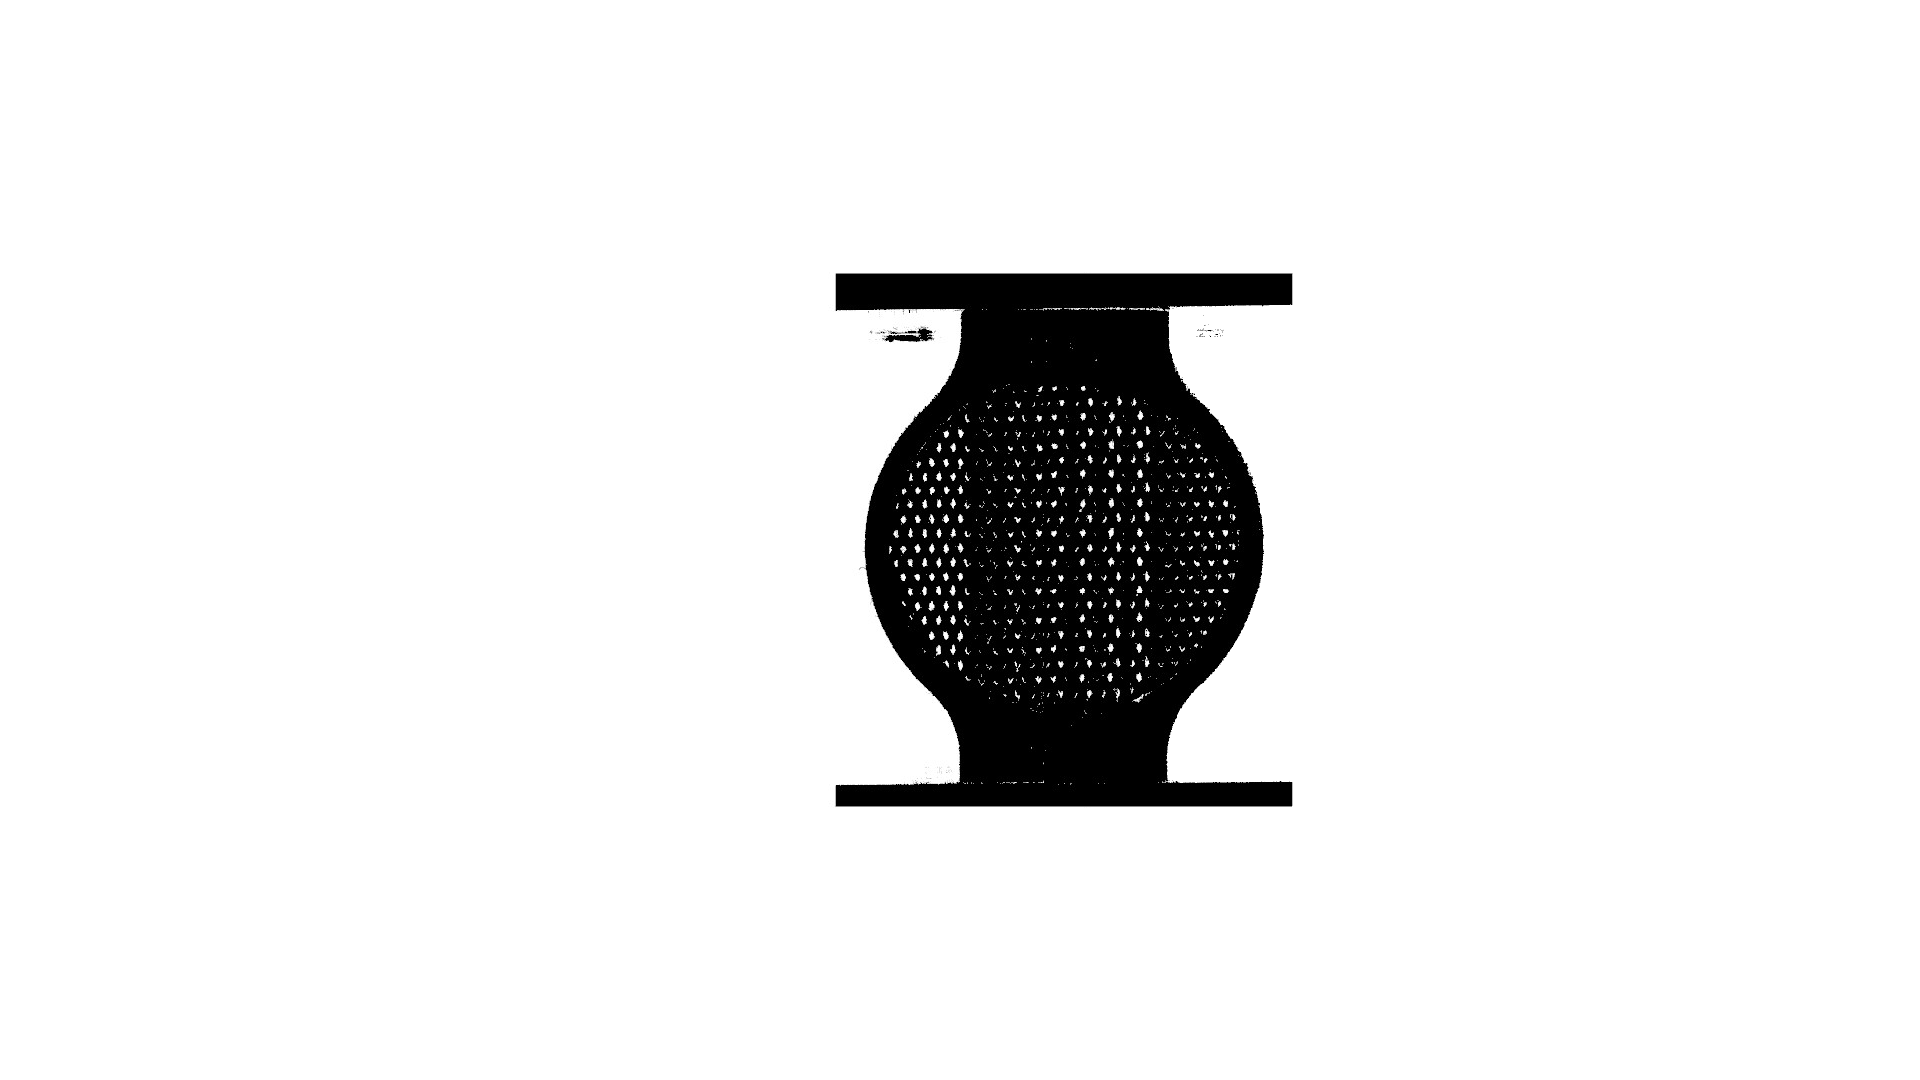
\includegraphics[height=150pt]{img_niklas/stichted.png}
        \caption[short]{Stichted image}
        %
      \end{figure}
    \end{minipage}
  \end{frame}

  \begin{frame}{Automatisierung}
    \begin{minipage}[h]{.6\textwidth}
        \begin{block}{Anforderungen:}
            \begin{itemize}
                \item Automatisierung
                \item Input: Scandateien, evtl orginale STL-Datei
                \item Output: Visueller Vergleich, Vergleichszahlen
                \item Validierung von verschiedenen Bauteilgeometrien 
                \item Universell auf Bauteile anwendbar.
                \item Einfach zu installierendes Programm.
            \end{itemize}
        \end{block}
    \end{minipage}
    \hfill
    \begin{minipage}[h]{.39\textwidth}
      
    \end{minipage}
  \end{frame}

  \begin{frame}{Ausblick}
    \begin{minipage}[h]{.6\textwidth}
        \begin{block}{Mögliche weitere Themen:}
            \begin{itemize}
                \item Vergleich von Materialen und Bauteilgeometrien
                \item 3D Vergleich anstelle von 2D Ansicht.
                \item Perfomance Verbesserungen des Algorithmus
            \end{itemize}
        \end{block}
    \end{minipage}
    \hfill
    \begin{minipage}[h]{.39\textwidth}       
    \end{minipage}
  \end{frame}
\end{document}